\documentclass[aps,prb,onecolumn,10pt,floatfix,superscriptaddress]{article} %pueden consultarse mas clases en 'REVTEX 4.1 Command and Options Summary'
%prb es la revista con las citas como superindices
%document class: article [twocolums,10pt,a4paper], book

\usepackage{listings}
\usepackage{amssymb} %amssymb y amsmath se usan juntos para ampliar
\usepackage{amsmath} %la cantidad de simbolos disponibles

\usepackage{graphicx} % permite usar imagenes fuera del modo dvi
\usepackage[spanish]{babel} % le dice al compilador que el idioma de escritura es espa\~nol
\usepackage[latin1]{inputenc} % permite usar caracteres de idiomas derivados del lat\'in
% \usepackage[T1]{fontenc} % permite usar acentos en el c\'odigo fuente

 \usepackage[pdftex,colorlinks=true,pdfstartview=FitH,linkcolor=blue,citecolor=blue,urlcolor=blue]{hyperref} % agrega hiperv\'inculos a la presentaci\'on en pdf

\usepackage[left=3cm,right=3cm,top=2cm,bottom=2cm]{geometry}
\renewcommand{\thefootnote}{\fnsymbol{footnote}}
%\usepackage[switch]{lineno} %Marca el n\'umero de linea... Poner \linenumbers donde se quiere empezar a contar
%\DeclareGraphicsExtensions{.pdf,.png,.jpg,.eps}%lo obvio

\begin{document}

\title{Pr\'actica $3$ : Memorias Asociativas}

\author{Melisa Maidana Capit\'an}

\date{Junio 2013} % se puede utilizar \today para que ponga autom\'aticamente la fecha

\maketitle 
%\tableofcontents
% 

\setlength{\parindent}{30pt}
\setlength{\parskip}{2.5ex plus 0ex minus 0ex}

\section*{Resumen}

El problema de memoria asociativa consiste en \textit{"Guardar en la red un conjunto de $p$ patrones $\xi^{\mu}_{i}$ de manera tal que cuando se le presente un nuevo patr\'on $\zeta_{i}$, la misma responda produciendo cualquiera de los patrones almacenados que m\'as se parezca a $\zeta_{i}$"}.

En el presente informe se muestran los resultados obtenidos para una red con el modelo de Hopfield con muchos patrones. Dado un n\'umero de neuronas $N$ y de patrones $p$, se seleccion\'o uno a uno cada patr\'on y se los dej\'o evolucionar seg\'un las reglas del modelo de Hopfield. Acontinuaci\'on se calcul\'o el overlap producido entre cada patr\'on y el resultante. Se calcul\'o la capacidad de carga para distintos valores de $N$ y $p$.

Luego se realiz\'o el mismo procedimeinto utilizando patrones obtenidos a partir de un modelo estad\'istico basado en sistemas magn\'eticos. En este caso, se utiliz\'o la aproximaci\'on de campo medio para difinir los estados neuronales.

\section{Redes de Hopfield}

Para la formulaci\'on de este modelo, se asume que los estados neuronales son "apagado" o "prendido", correspondientes a estados subumbrales o estados supraumbrales de la din\'amica neuronal. En este caso, los estados apagados son representados con el estado $-1$, mientras que los estados prendidos son representados con el estado $+1$. La din\'amica de la red est\'a dada por:

\begin{equation}
S_{i} := sgn (\sum^{N}_{j=1}\omega_{ij}S_{j}-\theta_{j}) 
\end{equation}

 donde $N$ es el n\'umero total de neuronas, $\omega_{ij}$ es el peso asignado a cada conexi\'on y $\theta_j$ es el valor del umbral de la j-\'esima neurona. Este \'ultimo puede omitirse agregando una neurona al sistema.

Seg\'un la "regla de Hebb", los pesos est\'an dados por $\omega_{ij} = \frac{1}{N} \sum^{p}_{\mu=1} \xi^{\mu}_{i} \xi^{\mu}_{j}$.

	donde $p$ es el n\'umero de patrones presentados.

Para analizar la estabilidad de un determinado patr\'on $\xi^{\nu}_{i}$ es necesario analizar:

\begin{equation}
sgn(h^{\nu}_{i}) = \xi^{\nu}_{i}
\end{equation}

donde la entrada de la unidad $i$ en el patr\'on $\nu$ es

\begin{equation}
h^{\nu}_{i} \equiv \sum_{j} \omega_{ij} \xi^{\nu}_{j} = \frac{1}{N} \sum_{j} \sum_{\mu} \xi^{\mu}_{i}\xi^{\mu}_{j}\xi^{\nu}_{j} = \xi^{\nu}_{i} + \frac{1}{N} \sum_{j} \sum_{\mu \neq \nu} \xi^{\mu}_{i}\xi^{\mu}_{j}\xi^{\nu}_{j}
\end{equation}

Si el segundo t\'ermino es peque\~no (menor que $1$), el mismo no modifica el valor que toma la funci\'on de transferencia a la neurona i-\'esima del patr\'on $\nu$ (dada por la funci\'on signo). Para valores peque\~nos de $p$, el segundo t\'ermino es suficientemente chico, de modo que los patrones almacenados son estables. Adem\'as, cualquier condiciones inicial cercana (en bits) al patr\'on $\xi^{\nu}_{i}$ converger\'a por efecto de la din\'amica del modelo, al patr\'on $\xi^{\nu}_{i}$.


\subsection{Modelado de una red de Hopfield}

Para programar una red de Hopfield se siguieron los siguientes pasos:

\begin{itemize}
\item  Se crearon patrones $\xi^{\mu}_{i}$ ($i=1...N;\mu = 1...p$) con valores equiprobables $\pm 1$.
\item  Se calcul\'o la matriz de conexciones $\omega_{ij} = \frac{1}{N} \sum^{p}_{\mu=1} \xi^{\mu}_{i} \xi^{\mu}_{j}$.
\item Se tom\'o un patr\'on como condici\'on inicial y se iter\'o la din\'amica hasta converger a $s^{\mu}_{i}$.
\item Se calcul\'o el overlap dado por $m^{\mu} = \frac{1}{N} \sum^{N}_{i=1} s^{\mu}_{i} \xi^{\mu}_{i}$.

\end{itemize}

Se program\'o una red de Hopfield para diferentes valores de $N$ y $p$, de manera que en algunos casos $p$ resulte lo suficientemente peque\~no para que los patrones sean puntos fijos de la din\'amica, y en otros de manera que no lo sean.

%==FIGURA======FIGURA======FIGURA======FIGURA======FIGURA======FIGURA=====
\begin{figure}[!htd] 
	\begin{minipage}[b]{0.450\linewidth}
   	    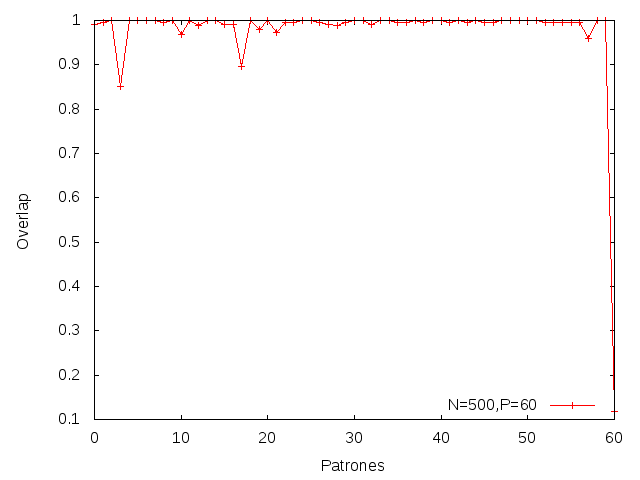
\includegraphics[scale=0.32 ]{12.png}
   	    \begin{center}
  \caption{\label{12} Overlap para $p/N = 0.12$ con $N=500$.}
     	    \end{center}
   \end{minipage}
   \begin{minipage}[b]{0.450\linewidth}
   	    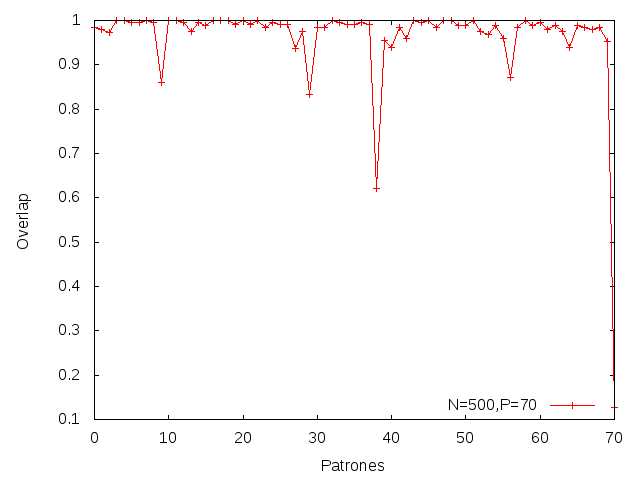
\includegraphics[scale=0.32 ]{14.png}
   	     \begin{center}
  \caption{\label{14} Overlap para $p/N = 0.14$ con $N=500$.}
     	    \end{center}
   \end{minipage}  
 \end{figure}
%==FIGURA======FIGURA======FIGURA======FIGURA======FIGURA======FIGURA=====

%==FIGURA======FIGURA======FIGURA======FIGURA======FIGURA======FIGURA=====
\begin{figure}[!htd] 
	\begin{minipage}[b]{0.450\linewidth}
   	    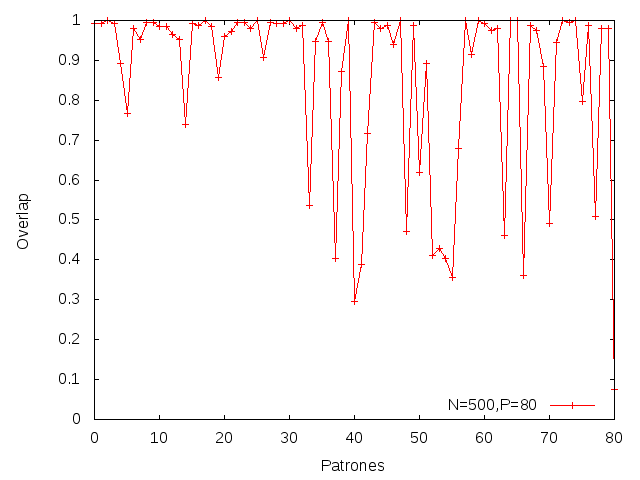
\includegraphics[scale=0.32 ]{16.png}
   	    \begin{center}
  \caption{\label{16} Overlap para $p/N = 0.16$ con $N=500$.}
     	    \end{center}
   \end{minipage}
   \begin{minipage}[b]{0.450\linewidth}
   	    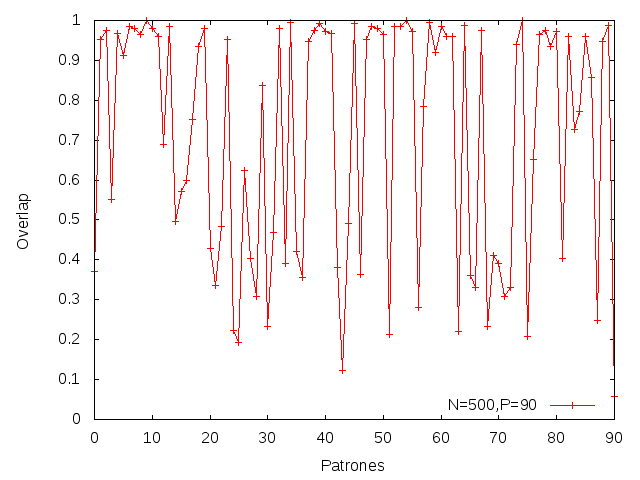
\includegraphics[scale=0.32 ]{18.png}
   	     \begin{center}
  \caption{\label{18}Overlap para $p/N = 0.18$ con $N=500$.}
     	    \end{center}
   \end{minipage} 
 \end{figure}
%==FIGURA======FIGURA======FIGURA======FIGURA======FIGURA======FIGURA=====

Se observa que a medida que el factor $\alpha = \frac{p}{N}$ aumenta, el overlap entre los patrones y el estado final de la din\'amica se vuelve m\'as peque\'no. Esto se corresponde al hecho de para algunos valores de $\alpha$ (suficientemente peque\~nos), los patrones resultan estables. El conjunto va perdiendo estabilidad conforme aumenta $\alpha$.

A continuaci\'on se presenta la distribuci\'on de overlap para diferentes valores de $\frac{p}{N}$.

\subsubsection{Distribuci\'on de overlap}


%==FIGURA======FIGURA======FIGURA======FIGURA======FIGURA======FIGURA=====
\begin{figure}[!htd] 
	\begin{minipage}[b]{0.450\linewidth}
   	    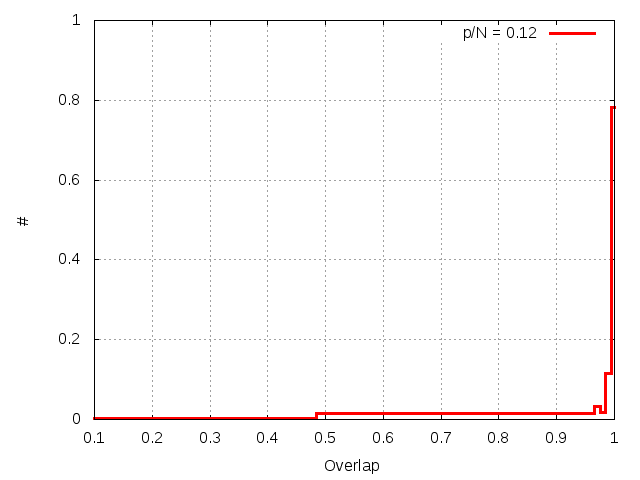
\includegraphics[scale=0.32 ]{Histo12.png}
   	    \begin{center}
  \caption{\label{Histo12} Distribuci\'on de overlap para $p/N = 0.12$ con $N=500$.}
     	    \end{center}
   \end{minipage}
   \begin{minipage}[b]{0.450\linewidth}
   	    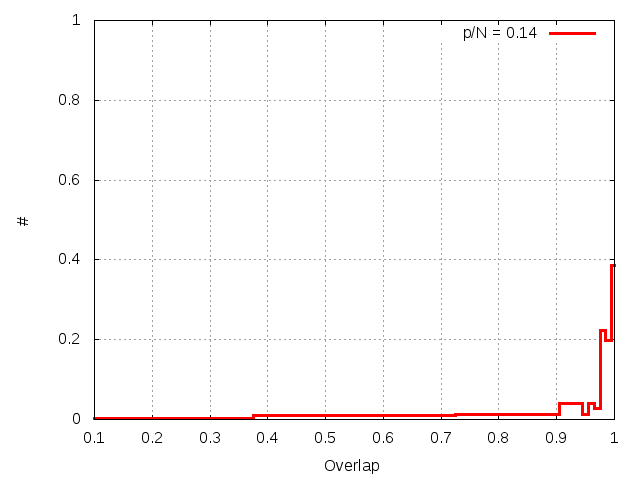
\includegraphics[scale=0.32 ]{Histo14.png}
   	     \begin{center}
  \caption{\label{Histo14} Distribuci\'on de overlap para $p/N = 0.14$ con $N=500$.}
     	    \end{center}
   \end{minipage}  
 \end{figure}
%==FIGURA======FIGURA======FIGURA======FIGURA======FIGURA======FIGURA=====

%==FIGURA======FIGURA======FIGURA======FIGURA======FIGURA======FIGURA=====
\begin{figure}[!htd] 
	\begin{minipage}[b]{0.450\linewidth}
   	    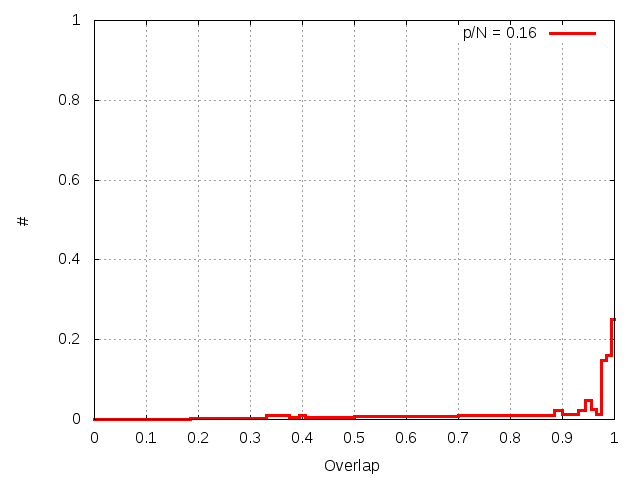
\includegraphics[scale=0.32 ]{Histo16.png}
   	    \begin{center}
  \caption{\label{Histo16} Distribuci\'on de overlap para $p/N = 0.16$ con $N=500$.}
     	    \end{center}
   \end{minipage}
   \begin{minipage}[b]{0.450\linewidth}
   	    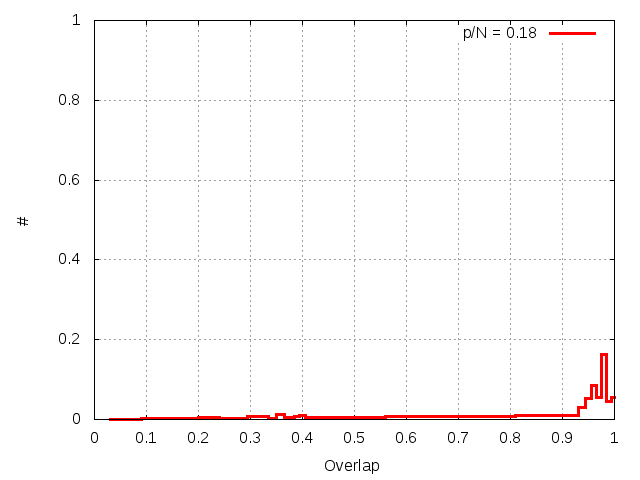
\includegraphics[scale=0.32 ]{Histo18.png}
   	     \begin{center}
  \caption{\label{Histo18} Distribuci\'on de overlap para $p/N = 0.18$ con $N=500$.}
     	    \end{center}
   \end{minipage} 
 \end{figure}
%==FIGURA======FIGURA======FIGURA======FIGURA======FIGURA======FIGURA=====

\section{Redes de Hopfield y Mec\'anica estad\'istica de modelos magn\'eticos}

El modelo de red de Hopfield se asemeja a algunos modelos simples de materiales magn\'eticos. En particular, el problema descripto anteriormente se asemeja al "Modelo de Ising", en el cu\'al los spines pueden tomar valores $\pm 1$. Los fuerza de las conexiones neuronales se asimilan a las fuerzas de intercambio de un material magn\'etico, y los umbrales son representados por el campo externo.

Supongase que ahora se reemplaza la regla determinista presentada anteriormente, por un modelo estoc\'astico dado por

\begin{equation}
\label{si}
S_{i} :=  
 \left\lbrace
 \begin{array}{l}
+1 $ con probabilidad $ p(h_i)\\
-1 $ con probabilidad $ 1-p(h_i)
\end{array}\right.
\end{equation}

donde ahora $p(h)$ depende de la temperatura. En este trabajo tomamos como distribuci\'on de probabilidad $p(h_i) = \frac{exp^{\beta h_i}}{exp^{\beta h_{i}}+exp^{-\beta h_{i}}}$.

En modelos magn\'eticos, este problema se resulve de manera aproximada mediante la \textit{teor\'ia de campo medio}. Esta aproximaci\'on consiste en reemplazar el valor de $h_{i}$ por su valor medio, de manera que 

\begin{equation}
\langle S_{i} \rangle = tanh (\beta \langle h_{i} \rangle)
\end{equation}

\subsection{Programaci\'on del modelo probabil\'istico}

Se program\'o una red con el modelo de Hopfield con estados neuronales dados por la funci\'on de probabilidad de la ec.(\ref{si}). Tomando uno de los patrones como condici\'on inicial se iter\'o un n\'umero $n = 10$ veces la din\'amica del modelo, y para cada patr\'on se calcul\'o el overlap. Se obtuvo el overlap medio para diferentes valores de temperatura $T$.

%==FIGURA======FIGURA======FIGURA======FIGURA======FIGURA======FIGURA=====
\begin{figure}[!htd] 
	\begin{minipage}[b]{0.450\linewidth}
   	    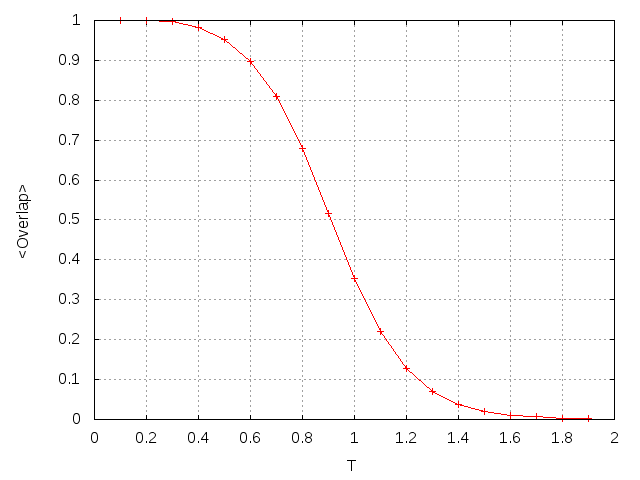
\includegraphics[scale=0.32 ]{Overlap2.png}
   	    \begin{center}
  \caption{\label{overlap2} .}
     	    \end{center}
   \end{minipage}
   \begin{minipage}[b]{0.450\linewidth}
   	    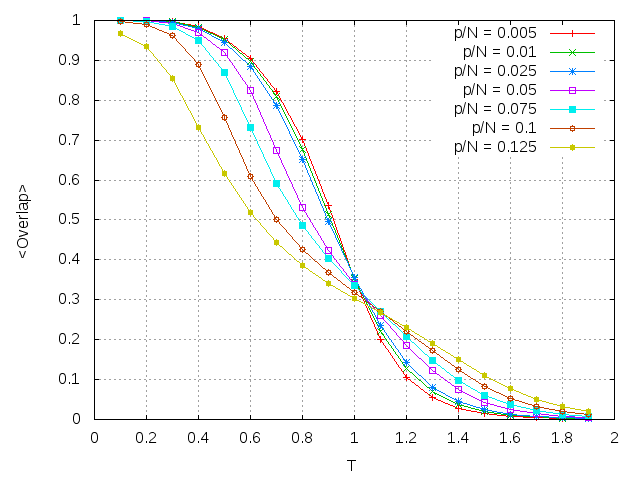
\includegraphics[scale=0.32 ]{Overlap_p.png}
   	     \begin{center}
  \caption{\label{overlap2b}}
     	    \end{center}
   \end{minipage} 
 \end{figure}
%==FIGURA======FIGURA======FIGURA======FIGURA======FIGURA======FIGURA=====

En la Fig.(\ref{overlap2}) se observan diferentes caracter\'isticas. En primer lugar, para valores $\frac{p}{N}$ suficientemente chicos, a temperaturas peque\~nas el overlap medio es practicamente $1$, y el mismo disminuye lentamente al aumentar $T$. En analog\'ia al sistema ferromagn\'etico, el estado de bajas temperaturas se corresponde a la tendencia de los spines a alinearse con el campo magn\'etico externo. En la red neuronal, significa que los patrones presentados son estables. Por otro lado, cuando la temperatura aumenta el ferromagneto se desordena y los spines apuntan en direcciones arbitrarias. En el caso de la red neuronal, el overlap medio se anula y esto se corresponde a la inestabilidad de los patrones.

En segundo lugar, se observa que la curva overlap medio vs. temperatura se modifica cuando cambia la relaci\'on $\frac{p}{N}$. 

\section{Programas en C}

\subsection{Programa Red de Hopfield determinista}
\begin{lstlisting}[frame=single,breaklines=true]

#include <stdlib.h>
#include <stdio.h>
#include <math.h>
#include <malloc.h>
#include <fstream>
#include <iostream>
#include <iostream>
#include <iomanip>
#include "nrutilc.h"
#include "funciones.h"

#include <cstdio>
#include <cstdlib>
#include <cmath>
#include <cstdio>
#include <cstdlib>
#include <cassert>
#include <malloc.h>

//include's de c++
#include <string>
#include <sstream>
using namespace std;

template<class T>
inline string to_string(const T& t){
    stringstream ss;
    ss << t;
    return ss.str();
}

int main(){

 int N,P;
 printf("Escriba el numero de neuronas de la red.\n");
 scanf("%d",&N);
 printf("Escriba el numero de patrones que desea almacenar\n");
 scanf("%d",&P);
		
 FILE *over;
 string red_overlap = to_string("Hopfield_overlap_") + to_string(N)+ to_string("_")+to_string(P)+to_string(".dat");
 if((over = fopen(red_overlap.c_str(), "w"))==NULL){
	printf("Problemas para abrir archivo overlap.dat");
	}
 MatInt patrones(N,P);
 srand(time(0));
 GeneraPatrones(patrones);
 MatDoub conexiones(N,N);
 MatConexiones(patrones,conexiones);
 VecDoub estados(N),estado_inicial(N);
 VecDoub overlap(P);
 VecDoub aux(N);
	
 for(int p=0;p<=P;p++){
 	for(int i=0;i<N;i++){
		estados[i]=patrones[i][p];
		estado_inicial[i]=patrones[i][p];
		}
	int conv=1;
	int convtime=0;
	while(conv != 0 && convtime<500){
		convtime++;
		conv=0;
		for(int i=0;i<N;i++)
			aux[i]=estados[i];
		Dinamica(estados,conexiones);
		for(int i=0;i<N;i++){
			if(estados[i]*aux[i]<0)
				conv=1;
			}
	}
	overlap[p] = CalculaOverlap(estados,estado_inicial);
	fprintf(over,"%lf\n", overlap[p]);
 } 
 fclose(over);
 return 0;
 }

\end{lstlisting}

\subsection{Programa Red de Hopfield estoc\'astico}
\begin{lstlisting}[frame=single,breaklines=true]

#define ITMAX 10
int main(){

 int N,P;
 printf("Escriba el numero de neuronas de la red.\n");
 scanf("%d",&N);
 printf("Escriba el numero de patrones que desea almacenar\n");
 scanf("%d",&P);
		
 FILE *over;
 string red_overlap = to_string("Hopfield2_overlapmedio_") + to_string(N)+ to_string("_")+to_string(P)+to_string(".dat");
 if((over = fopen(red_overlap.c_str(), "w"))==NULL){
	printf("Problemas para abrir archivo overlap.dat");
	}
	
 MatInt patrones(N,P);
 srand(time(0));
 GeneraPatrones(patrones);
 MatDoub conexiones(N,N);
 MatConexiones(patrones,conexiones);

 VecDoub estados(N),estado_inicial(N);
 VecDoub overlap(P);
 VecDoub aux(N);
 VecDoub h(N);
 MatDoub prob(N,2);
 double beta;
 double TMAX=2;
 double temperature=0.1;
 double overlap_medio;
	
 while(temperature<=TMAX){
 	cout << t << endl;
	for(int p=0;p<=P;p++){
		for(int i=0;i<N;i++){
			estados[i]=patrones[i][p];
			estado_inicial[i]=patrones[i][p];
			}
		int iteraciones=0;
		while(iteraciones < ITMAX){
			CalculaH(conexiones,estados,h);
			beta=1./temperature;
			CalculaProb(h,prob,beta);
			DinamicaProb(prob,estados);
			iteraciones++;
		}
		overlap[p] = CalculaOverlap(estados,estado_inicial);
		}
	overlap_medio=PromVector(overlap);	
	fprintf(over,"%lf\t%lf\n", temperature ,overlap_medio);
	temperature+=0.1;
	}
	
 fclose(over);
 return 0;
 }

\end{lstlisting}

\subsection{Librer\'ia auxiliar}

\begin{lstlisting}[frame=single,breaklines=true]

#ifndef FUNCIONESINT_H
#define FUNCIONESINT_H

void GeneraPatrones(MatInt &matrix);
void MatConexiones(MatInt &matrix,MatDoub &Conexiones);
int Signo(double x);
void Dinamica(VecDoub &estados,MatDoub &conexiones);
double CalculaOverlap(VecDoub &efinal,VecDoub &einicial);
void CalculaH(const MatDoub &conexiones,const VecDoub &estados,VecDoub &h);
void CalculaProb(const VecDoub &h,MatDoub &prob,double beta);
void DinamicaProb(const MatDoub &prob,VecDoub &estados);
double PromVector(const VecDoub &vector);

void GeneraPatrones(MatInt &matrix){
	
 int p=matrix.ncols();
 int n=matrix.nrows();
	
 double aleatorio;
 for(int i=0;i<n;i++){
	for(int j=0;j<p;j++){
		aleatorio = rand()*1./RAND_MAX;
		if(aleatorio > 0.5)
			matrix[i][j] = 1;
		else
			matrix[i][j] = -1;
		}
	}
}
void MatConexiones(MatInt &matrix,MatDoub &Conexiones){
	
 int n = matrix.nrows();
 int m = matrix.ncols();
	
 for(int i=0;i<n;i++){
	for(int j=0;j<i;j++){
		for(int k=0;k<m;k++)
			Conexiones[i][j]+=matrix[i][k]*matrix[j][k];
		Conexiones[i][j]/=n;
		}
	}
	
 for(int i=0;i<n;i++){
	for(int j=i;j<n;j++){
		Conexiones[i][j]=Conexiones[j][i];
		}
	}
	
 for(int i=0;i<n;i++){
	Conexiones[i][i]=0;
	}
}	
int Signo(double x){
 if(x>0)
	return 1;
 else
	return -1;
}
	
void Dinamica(VecDoub &estados,MatDoub &conexiones){
	
 int n = estados.size();
 VecDoub auxiliar(n);

 for(int i=0;i<n;i++){
	auxiliar[i]=estados[i];
	estados[i]=0;	
	}
	
 for(int i=0;i<n;i++){
	for(int j=0;j<n;j++)
		estados[i]+=conexiones[i][j]*auxiliar[j];
	estados[i]=Signo(estados[i]);
	}	
}
double CalculaOverlap(VecDoub &efinal,VecDoub &einicial){
	
 double mu,suma=0;
 int n=efinal.size();

 for(int i=0;i<n;i++)
	suma+=efinal[i]*einicial[i];
 mu = suma*1.0/n;
 return mu;
}	
void CalculaH(const MatDoub &conexiones,const VecDoub &estados,VecDoub &h){
	
 int n=h.size();
	
 for(int i=0;i<n;i++)
	h[i]=0;
	
 for(int i=0;i<n;i++){
	for(int j=0;j<n;j++){
		h[i]+=conexiones[i][j]*estados[j];
	}
 }
}

void CalculaProb(const VecDoub &h,MatDoub &prob,double beta){
	
 int n=h.size();
	
 for(int i=0;i<n;i++){
	prob[i][0]=exp(beta*h[i])/(exp(beta*h[i])+exp(-beta*h[i]));
	prob[i][1]=exp(-beta*h[i])/(exp(beta*h[i])+exp(-beta*h[i]));		
	}
 }	
void DinamicaProb(const MatDoub &prob,VecDoub &estados){
	
 int n=estados.size();
	
 for(int i=0;i<n;i++){
	estados[i]=1*prob[i][0]+(-1)*prob[i][1];
 }
}

double PromVector(const VecDoub &vector){
	
 int n=vector.size();
 double prom=0;
	
 for(int i=0;i<n;i++)
	prom+=vector[i];
 prom/=n;
 return prom;
}
#endif


\end{lstlisting}


\begin{thebibliography}{99}

\bibitem IIntroduction to the theory of neural computation. John Hertz,Anders Krogh,Richard G.Palmer. Westview Press (1991).

\end{thebibliography}



\end{document}